\documentclass{zkdl-presentation-template}

\title[Bulletproofs: inner-product argument]{\textbf{Bulletproofs: inner-product argument}}
\author{Distributed Lab}
\date{July 24, 2025}
\homepage{zkdl-camp.github.io}
\github{ZKDL-Camp}

\pgfplotsset{compat=1.18}

\begin{document}
\frame {
    \tikz [remember picture,overlay]
    \node at
    ([yshift=1.5cm,xshift=-1.5cm]current page.south east)
%or: (current page.center)
        {
\includegraphics[width=60pt]{images/logo.png}};

    \titlepage
}

\begin{frame}{Plan}
    \tableofcontents
\end{frame}

\section{Introduction}

\begin{frame}{Bulletproofs: just some basic linear algebra}
    \begin{figure}[h!]
        \centering
        
\includegraphics[width=0.7\textwidth]{images/lecture_14/meme.jpg}
    \end{figure}
\end{frame}

\begin{frame}{Bulletproofs: Motivation}
    \begin{itemize}
        \item \textbf{Bulletproofs:} zero-knowledge proofs with logarithmic proof size
        \item No trusted setup, just some basic linear algebra
        \item Straightforward cryptographic assumption: discrete logarithm without bilinear pairings or other advanced assumptions
        \item Originally developed for efficient range proofs in confidential transactions
        \item Applicable for proving arithmetic circuits satisfiability (e.g., R1CS)
        \item Efficient polynomial commitment scheme could be derived (e.g., \textit{IPA} polynomial commitment)
        \item Heart of \textit{bulletproofs} -- \textbf{inner-product argument}
    \end{itemize}
\end{frame}

\begin{frame}{Bulletproofs: Building blocks}
    \begin{itemize}
        \item Zero-knowledge multiplication protocol \textbf{zk-mul}
        \item Inner-product argument \textbf{IPA}
        \item Application: \textit{IPA} polynomial commitment scheme
        \item Application: range proofs
        \item Application: arithmetic circuits satisfiability
    \end{itemize}
\end{frame}

\begin{frame}{Preliminaries}
    \begin{itemize}
        \item $\mathbb{G}$ -- cyclic group of prime order $p$ where \textbf{DLog} assumption holds
        \item $G, B \in \mathbb{G}$ -- independent generators
        \item $\mathbf{G}, \mathbf{H} \in \mathbb{G}^n$ -- vectors of generators with mutually unknown discrete log relations
        \item $\langle \mathbf{a}, \mathbf{b} \rangle = \sum_{i=1}^n a_i b_i$ -- inner product of scalar vectors $\mathbf{a}, \mathbf{b} \in \mathbb{F}_p^n$
        \item $\langle \mathbf{a}, \mathbf{G} \rangle = \sum_{i=1}^n [a_i] G_i$ -- inner product of a scalar vector $\mathbf{a} \in \mathbb{F}_p^n$ with a vector of generators $\mathbf{G} \in \mathbb{G}^n$
        \item $\mathbf{k}^n = (1, k, k^2, \dots, k^{n-1})$
    \end{itemize}
\end{frame}

% --- Next Sections ---

\section{Zero-knowledge multiplication}

\begin{frame}{Zero-knowledge multiplication}
    \textbf{Goal:} Prove knowledge of $a, b \in \mathbb{F}_p$ such that $c = ab$ without revealing $a, b, c$, i.e. consider the relation:
    $$\mathcal{R}_{abc} = \{ (\bot;c,a,b) \mid c=ab \}$$
    Curious reader could argue that this is relatively simple problem as we have $\Sigma$-protocols framework, especially Chaum-Pedersen protocol for DH-triplets, e.g. we could prove slightly modified relation:
    $$\mathcal{R}'_{abc} = \{ (P, Q_a, Q_b, Q_c \in \mathbb{G};a,b) \mid Q_c = [a]Q_b, Q_a = [a]P, Q_b = [b]P \}$$
    
    \begin{alertblock}{Problem}
        Prover does not hide $a,b,c$ values so that adversary could potentially learn them if they are values especially if they are small or have non-uniform distribution.
    \end{alertblock}
\end{frame}

\begin{frame}{Multiplication of committed values}
    \begin{block}{Solution}
        Use Pedersen commitments to bind to $a,b,c$ values.
    \end{block}
    $$
        \mathcal{R}'_{abc} = \left\{\begin{array}{l}
            (G,H,B,A,V; a,b, \alpha, \beta \in \mathbb{F}_p) \mid \\
            V = [ab]G + [\beta]B, \\
            A = [a]G + [b]H + [\alpha]B
        \end{array}\right\}
    $$
    Here $A$ is a binding Pedersen commitment to both $a$ and $b$ while $V$ is a binding Pedersen commitment to their product $ab$.
    \begin{alertblock}{Problem}
        How to prove that in zero-knowledge?
    \end{alertblock}
\end{frame}

\begin{frame}{Zero-knowledge polynomial multiplication}
    In order to provide zero-knowledge proof of $\mathcal{R}'_{abc}$ we bring out polynomials!
    \begin{align*}
        l(x) &= a + s_L x\\
        r(x) &= b + s_R x\\
        t(x) &= l(x)r(x) = ab + (s_L + s_R)bx + s_Ls_Rx^2
    \end{align*}
    What we have now:
    \begin{itemize}
        \item $s_L, s_R \in \mathbb{F}_p$ are blinding factors
        \item $l(x)$ is a linear polynomial hiding value $a$
        \item $r(x)$ is a linear polynomial hiding value $b$
        \item $t(x)$ is a quadratic polynomial, constant term is the product $ab$, the product we typically want to prove knowledge of.
    \end{itemize}
\end{frame}

\begin{frame}{Zero-knowledge polynomial multiplication}
    \begin{block}{Idea}
        If $l(x)r(x) = t(x)$ than with high probability for random $u \in \mathbb{F}_p$ we have $l(u)r(u) = t(u)$ due to \textit{Schwartz-Zippel lemma}
    \end{block}
    Now we can build a zero-knowledge protocol \textbf{zk-mul} for proving a product of degree-one polynomials $l(x)r(x) = t(x)$:
    \begin{itemize}
        \item Prover computes and sends to $\mathcal{V}$ commitments to coefficients of $l(x), r(x), t(x)$:
            \begin{align*}
                A &= [a]G + [b]H + [\alpha]B & T_0 &= [ab]G + [\tau_0]B\\
                S &= [s_L]G + [s_R]H + [\beta]B &T_1 &= [s_L + s_R]G + [\tau_1]B\\
                &&T_2 &= [s_Ls_R]G + [\tau_2]B
            \end{align*}
        Here $A$ -- commitment to constant terms, $S$ -- commitment to degree-one coefficients of $l(x),r(x)$, $T_{i}$ for $i=0..2$ -- commitments to coefficients of $t(x)$.
    \end{itemize}
\end{frame}

\begin{frame}{Zero-knowledge polynomial multiplication}
    \begin{itemize}
        \item Verifier draws random challenge $u \in \mathbb{F}_p$ and sends it to prover
        \item Prover evaluates and sends to Verifier $(l_u, r_u, t_u, \alpha_u, \tau_u)$: 
        \begin{align*}
            l_u &=l(u), r_u = r(u), t_u = t(u) = l_u \cdot r_u, \\
            \alpha_u &= \alpha + \beta u, \tau_u = \tau_0 + \tau_1 u + \tau_2 u^2
        \end{align*}
        \item Verifier checks:
        \begin{align*}
            A + [u]S &\stackrel{?}{=} [l_u]G + [r_u]H + [\alpha_u]B \\
            [t_u]G + [\tau_u]B &\stackrel{?}{=} T_0 + [u]T_1 + [u^2]T_2 \\
            t_u &\stackrel{?}{=} l_u r_u
        \end{align*}
    \end{itemize}
\end{frame}

\begin{frame}{Zero-knowledge numbers multiplication}
    Now we could easily tweak our \textbf{zk-mul} protocol to prove relation     
    $$
    \mathcal{R}'_{abc} = \left\{\begin{array}{l}
        (G,H,B,A,V; a,b, \alpha, \beta \in \mathbb{F}_p) \mid \\
        V = [ab]G + [\beta]B, \\
        A = [a]G + [b]H + [\alpha]B
    \end{array}\right\}
    $$ 
    in zero-knowledge: just use prescribed commitment $A$ as a commitment to constant terms of $l(x), r(x)$ and $V$ as a commitment $T_0$ to constant coefficient of $t(x)$
\end{frame}

\begin{frame}{zk-mul protocol: Security}
    \begin{theorem}
        Zero-knowledge polynomial multiplication protocol \textbf{zk-mul} is perfect complete, special sound and perfect honest-verifier zero-knowledge.
    \end{theorem}
    Here we briefly show the completeness:
    \begin{itemize}
        \item First check: \begin{align*}
            A + [u]S &\stackrel{?}{=} [l_u]G + [r_u]H + [\alpha_u]B \\
            LHS &= [a]G + [b]H + [\alpha]B + [us_L]G + [us_R]H + [u\beta]B \\
            RHS &= [a+ u s_L]G + [b + u s_R]H + [\alpha + u \beta]B = \\
            &=[a]G + [b]H + [\alpha]B + [us_L]G + [us_R]H + [u\beta]B
        \end{align*}
        As $LHS = RHS$ the check is satisfied.
    \end{itemize}
\end{frame}

\begin{frame}{zk-mul protocol: Security}
    \begin{itemize}
        \item Second check: \begin{align*}
            [t_u]G + [\tau_u]B &\stackrel{?}{=} T_0 + [u]T_1 + [u^2]T_2 \\
            LHS &= [ab + t_1 u + t_2 u^2]G + [\tau_0 + \tau_1 u + \tau_2 u^2]B\\
            RHS &=[ab]G + [\tau_0]B + [u]([t_1]G + [\tau_1]B) + \\
            &+ [u^2]([t_2]G + [\tau_2]B)
        \end{align*}
        As $LHS = RHS$ the check is satisfied.
        \item The third check is $t_u = l_u r_u$ holds by definition
    \end{itemize}
    Intuitively \textbf{zk-mul} protocol is also \textit{zero-knowledge} as it is easy to simulate every step of the honest prover. \textit{Special soundness} holds as it's easy to build an extractor similar to Okamoto's protocol extractor for extracting openings of Pedersen commitments.
\end{frame}

\begin{frame}{zk-mul: inner-product version}
    We could easily generalize \textbf{zk-mul} protocol to prove $t(x) = \langle \mathbf{l}(x), \mathbf{r}(x) \rangle $ for polynomials with vector coefficients $\mathbf{l}(x), \mathbf{r}(x), \mathbf{t}(x) \in \mathbb{F}_p^n[x]$. Specifically using generalized \textbf{zk-mul} protocol we could also prove in zero-knowledge that inner-product relation holds for vectors $\mathbf{a}, \mathbf{b} \in \mathbb{F}_p^n$:
    \begin{align*}
        \mathcal{R}_{zkip} = \left\{ \begin{aligned} (\mathbf{G,H},G,B,A,V;\mathbf{a,b},\alpha, \gamma) \vert & A = \langle \mathbf{a,G} \rangle + \langle \mathbf{b,H} \rangle + [\alpha] B, \\ & V = [\langle \mathbf{a,b} \rangle]G + [\gamma]B \end{aligned} \right\}
    \end{align*}
    \begin{alertblock}{Problem}
        Proof size is linear in $n$ as the prover should send evaluated vectors $\mathbf{l_u}, \mathbf{r_u}$. We will adress this problem in the next section: \textbf{inner-product argument}.
    \end{alertblock}
\end{frame}

\section{Inner-product argument}

\begin{frame}{Motivation: Inner-product Argument}
    The heart of \textbf{bulletproofs} is \textbf{inner-product argument(IPA)} which allows to soundly prove inner-product relation between two vectors $\mathbf{a}, \mathbf{b} \in \mathbb{F}_p^n$:
    $$\mathcal{R}_{ip} = \{ (\mathbf{G,H}, P, c; \mathbf{a,b}) \vert P = \langle \mathbf{a,G} \rangle + \langle \mathbf{b,H} \rangle \wedge \langle \mathbf{a,b} \rangle = c \}$$
    Firstly, let's combine statements $P = \langle \mathbf{a,G} \rangle + \langle \mathbf{b,H} \rangle \wedge \langle \mathbf{a,b} \rangle = c$ into a single statement by multiplying the second one by a random challenge $r \in \mathbb{F}_p$ and some orthogonal generator $B \in \mathbb{G}$, summing up:
    $$
    \mathcal{R}'_{ip} = \{ (\mathbf{G,H}, Q, P'; \mathbf{a,b}) \vert P' = \langle \mathbf{a,G} \rangle + \langle \mathbf{b,H} \rangle + [\langle \mathbf{a,b} \rangle]Q \}
    $$
    Where $Q=[r]B, P' = P + [cr]B = P+[c]Q$
\end{frame}

\begin{frame}{Compression step}
    Assuming $n = 2^d$ define by $\mathbf{G_{lo}} = (G_1, \dots, G_{n/2}), \mathbf{G_{hi}} = (G_{n/2+1},\dots, G_n) \in \mathbb{G}^{n/2}$ -- lower and higher halves of vector $\mathbf{G}$ and $\mathbf{a_{lo}} = (a_1, \dots, a_{n/2}), \mathbf{a_{hi}} = (a_{n/2+1},\dots,a_n) \in \mathbb{F}_p^{n/2}$ -- lower and higher halves of $\mathbf{a} \in \mathbb{F}_p^{n}$.

    Let $u_k \in \mathbb{F}_p$ - be challenge scalar, define compressed vectors:
    \begin{align*}
        \mathbf{a}^{(k-1)} &= \mathbf{a_{lo}} \cdot u_k + u_k^{-1} \cdot \mathbf{a_{hi}} \\
        \mathbf{b}^{(k-1)} &= \mathbf{b_{lo}} \cdot u_k^{-1} + u_k \cdot \mathbf{b_{hi}} \\
        \mathbf{G}^{(k-1)} &= \mathbf{G_{lo}} \cdot u_k^{-1} + u_k \cdot \mathbf{G_{hi}} \\
        \mathbf{H}^{(k-1)} &= \mathbf{H_{lo}} \cdot u_k + u_k^{-1} \cdot \mathbf{H_{hi}}
    \end{align*}
    \vspace{-1em}
    \begin{alertblock}{Note}
        If $n$ is not a power of two we could pad vectors with zeroes to the next power of two.
    \end{alertblock}
\end{frame}

\begin{frame}{Compression step: illustration}
    \begin{figure}[h!]
        \centering
        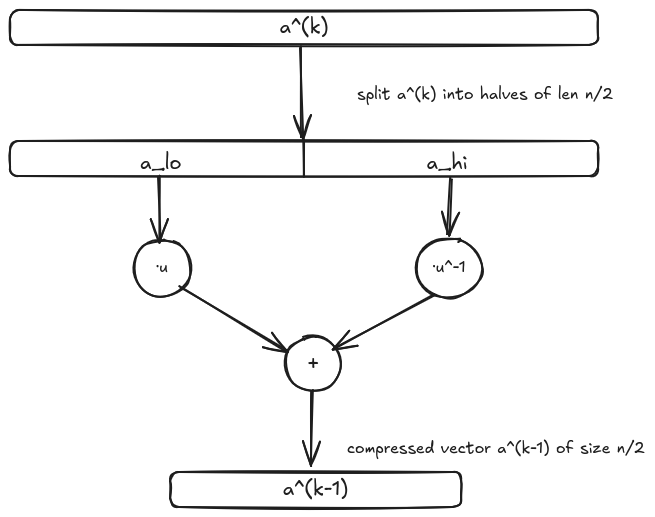
\includegraphics[width=0.8\textwidth]{images/lecture_14/compressed.png}
        \label{fig:compression}
    \end{figure}
\end{frame}

\begin{frame}{Commitment compression}
    Define $P_k \gets P' =  \langle \mathbf{a,G} \rangle + \langle \mathbf{b,H} \rangle + [\langle \mathbf{a,b} \rangle]Q$ -- current commitment to vectors $\mathbf{a,b}$ and define $P_{k-1}$ using compressed vectors to have the same form as $P_k$, but in new basis $(\mathbf{G}^{(k-1)}, \mathbf{H}^{(k-1)})$:
    \begin{equation*}
        P_{k-1} = \langle \mathbf{a}^{(k-1)}, \mathbf{G}^{(k-1)} \rangle + \langle \mathbf{b}^{(k-1)}, \mathbf{H}^{(k-1)} \rangle + [\langle \mathbf{a}^{(k-1)}, \mathbf{b}^{(k-1)} \rangle]Q
    \end{equation*}
    Substituting compressed vectors and applying bilinearity property of inner product we get:
\begin{align*}
    P_{k-1} = & \textcolor{Blue}{\langle \mathbf{a_{lo}}, \mathbf{G_{lo}}\rangle + \langle \mathbf{a_{hi}}, \mathbf{G_{hi}}\rangle} &+ \textcolor{Peach}{u_k^2\langle \mathbf{a_{lo}}, \mathbf{G_{hi}}\rangle} + \textcolor{ForestGreen}{u_k^{-2}\langle \mathbf{a_{hi}}, \mathbf{G_{lo}}\rangle} + \\
    & \textcolor{Blue}{\langle \mathbf{b_{lo}}, \mathbf{H_{lo}}\rangle + \langle \mathbf{b_{hi}}, \mathbf{H_{hi}}\rangle} &+ \textcolor{Peach}{u_k^2\langle \mathbf{b_{hi}}, \mathbf{H_{lo}}\rangle} + \textcolor{ForestGreen}{u_k^{-2}\langle \mathbf{b_{lo}}, \mathbf{H_{hi}}\rangle} + \\
    & \textcolor{Blue}{[\langle \mathbf{a_{lo}}, \mathbf{b_{lo}}\rangle + \langle \mathbf{a_{hi}}, \mathbf{b_{hi}}\rangle]Q} &+ \textcolor{Peach}{[u_k^2\langle \mathbf{a_{lo}}, \mathbf{b_{hi}}\rangle} + \textcolor{ForestGreen}{u_k^{-2}\langle \mathbf{a_{hi}}, \mathbf{b_{lo}}\rangle]Q}
\end{align*}
The first two columns precisely represent current commitment $P_k$, for the last two columns we define $L_k, R_k$ as commitments to cross terms
\end{frame}

\begin{frame}{Commitment compression}
    So that we represent new commitment $P_{k-1}$ from the old one $P_k$ and cross terms $L_k, R_k$:
    \begin{align*}
        P_{k-1} &= \textcolor{Blue}{P_k} + \textcolor{Peach}{[u_k^2] L_k} + \textcolor{ForestGreen}{[u_k^{-2}] R_k} \\
        L_{k} &= \langle \mathbf{a_{lo}}, \mathbf{G_{hi}}\rangle + \langle \mathbf{b_{hi}}, \mathbf{H_{lo}}\rangle + [\langle \mathbf{a_{lo}}, \mathbf{b_{hi}}\rangle]Q \\
        R_{k} &= \langle \mathbf{a_{hi}}, \mathbf{G_{lo}}\rangle + \langle \mathbf{b_{lo}}, \mathbf{H_{hi}}\rangle + [\langle \mathbf{a_{hi}}, \mathbf{b_{lo}}\rangle]Q
    \end{align*}
    So the basic logic of compression step:
    \begin{itemize}
        \item Verifier draws challenge $u_k \xleftarrow{R} \mathbb{F}_p$ and sends it to prover
        \item Prover computes $\mathbf{a}^{(k-1)}, \mathbf{b}^{(k-1)}$ and $L_k, R_k$ and sends them to verifier
        \item Verifier reconstructs $P_{k-1}$ using $\mathbf{a}^{(k-1)}, \mathbf{b}^{(k-1)}$ and checks:
        $$P_{k-1} = P_k + [u_k^2] L_k + [u_k^{-2}] R_k$$
    \end{itemize}
        
\end{frame}

\begin{frame}{Recursive compression}
    \begin{block}{Remark}
        We wish not send $\mathbf{a}^{(k-1)}, \mathbf{b}^{(k-1)}$ directly as this's inefficient due to still linear sizes, instead we apply recursion to compress this vectors to just one element. 
    \end{block}
    Here we come up with some kind of statement compression algorithm reducing size of all vectors in half per compression step. Repeating compression algorithm $k$ times we end up with sending vectors $\mathbf{a}^{(0)}, \mathbf{b}^{(0)}$ each of length one and $P_0$ containing all accumulated cross-terms:
    \begin{align*}
        P_0 &= [a_1^{(0)}]G_1^{(0)} + [b_1^{(0)}]H_1^{(0)} + [a_1^{(0)}b_1^{(0)}]Q \\
        P_0 &= P_k + \sum_{i=1}^k ([u_i^2]L_i + [u_i^{-2}]R_i)
    \end{align*}
    Verifier compares this $P_0$s and asserts inner-product correctness.
\end{frame}

\begin{frame}{Inner-product argument protocol}
    Here we describe the \textbf{inner-product argument} protocol between prover $\mathcal{P}$ and verifier $\mathcal{V}$ for relation $\mathcal{R}'_{ip} = \{ (\mathbf{G,H}, Q, P'; \mathbf{a,b}) \vert P' = \langle \mathbf{a,G} \rangle + \langle \mathbf{b,H} \rangle + [\langle \mathbf{a,b} \rangle]Q \}$ from scratch.
    \begin{itemize}
        \item Prover $\mathcal{P}$ sets $$(k, \mathbf{a}^{(k)}, \mathbf{b}^{(k)}, \mathbf{G}^{(k)}, \mathbf{H}^{(k)}, P_k) \gets (d, \mathbf{a,b,G,H},P')$$
        \item Verifier $\mathcal{V}$ sets $$(k, \mathbf{G}^{(k)}, \mathbf{H}^{(k)}, P_k) \gets (d, \mathbf{G,H},P')$$
        \item While $k > 0$ then parties involve in \textbf{compression step protocol}
    \end{itemize}
\end{frame}

\begin{frame}{Compression step protocol}
    \begin{itemize}
        \item Prover $\mathcal{P}$ computes and sends to $\mathcal{V}$
            \begin{align*}
                L_{k} &= \langle \mathbf{a_{lo}}^{(k)}, \mathbf{G_{hi}}^{(k)}\rangle + \langle \mathbf{b_{hi}}^{(k)}, \mathbf{H_{lo}}^{(k)}\rangle + [\langle \mathbf{a_{lo}}^{(k)}, \mathbf{b_{hi}}^{(k)}\rangle]Q \\
                R_{k} &= \langle \mathbf{a_{hi}}^{(k)}, \mathbf{G_{lo}}^{(k)}\rangle + \langle \mathbf{b_{lo}}^{(k)}, \mathbf{H_{hi}}^{(k)}\rangle + [\langle \mathbf{a_{hi}}^{(k)}, \mathbf{b_{lo}}^{(k)}\rangle]Q
            \end{align*}
        \item $\mathcal{V}$ draws challenge $u_k \xleftarrow{R} \mathbb{F}_p$ and sends it to $\mathcal{P}$
        \item Both $\mathcal{P}$ and $\mathcal{V}$ compute:
            \begin{align*}
                \mathbf{G}^{(k-1)} &= \mathbf{G_{lo}}^{(k)} \cdot u_k^{-1} + u_k \cdot \mathbf{G_{hi}}^{(k)} \\
                \mathbf{H}^{(k-1)} &= \mathbf{H_{lo}}^{(k)} \cdot u_k + u_k^{-1} \cdot \mathbf{H_{hi}}^{(k)}
            \end{align*}
        \item $\mathcal{P}$ computes:
            \begin{align*}
                \mathbf{a}^{(k-1)} &= \mathbf{a_{lo}}^{(k)} \cdot u_k + u_k^{-1} \cdot \mathbf{a_{hi}}^{(k)} \\
                \mathbf{b}^{(k-1)} &= \mathbf{b_{lo}}^{(k)} \cdot u_k^{-1} + u_k \cdot \mathbf{b_{hi}}^{(k)} \\
            \end{align*}
    \end{itemize}
\end{frame}

\begin{frame}{Final step}
    At the final step when $k=0$ parties perform final check:
    \begin{itemize}
        \item Prover $\mathcal{P}$ sends $(a,b) \gets (\mathbf{a}_1^{(0)}, \mathbf{b}_1^{(0)})$ to verifier $\mathcal{V}$
        \item Verifier performs final check: 
            $$P' + \sum_{i=1}^d ([u_i^2]L_i + [u_i^{-2}]R_i) = [a]G_1^{(0)} + [b]H_1^{(0)} + [ab]Q$$
        outputs \textbf{accept} if equality holds and \textbf{reject} otherwise.
    \end{itemize}
\end{frame}

\begin{frame}{Inner-product argument: illustration}
    \begin{figure}[h!]
        \centering
        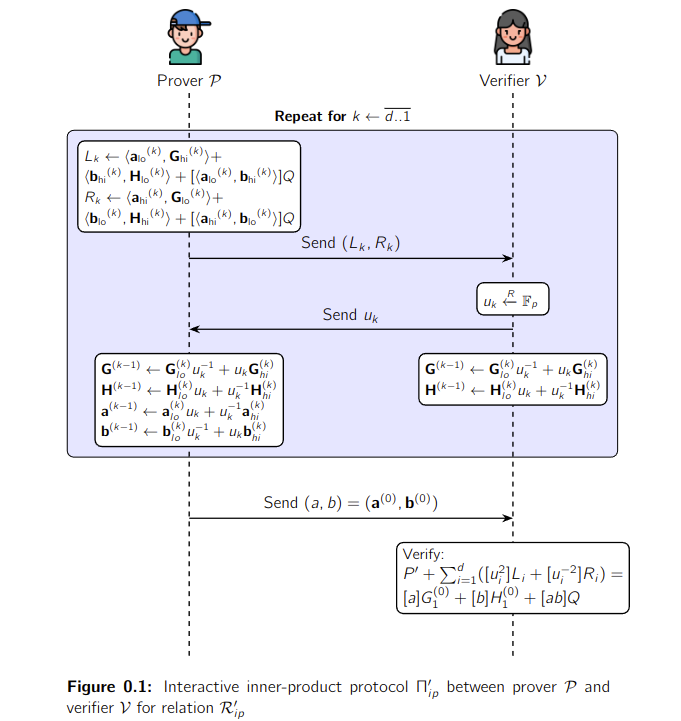
\includegraphics[width=0.8\textwidth]{images/lecture_14/ipa.png}
        \label{fig:ipa}
    \end{figure}
\end{frame}

\begin{frame}{Inner-product argument: security \& performance}
    \begin{block}{Remark}
        Overall communication complexity of \textbf{inner-product argument} is $2\log_2 n$ group elements plus $2$ field elements so we come up with logarithmic proof size for our inner-product relation $\mathcal{R}_{ip}$.
    \end{block}
    \begin{theorem}[Inner-Product Argument]
        The \textbf{inner-product argument} for relation $\mathcal{R}_{ip}$ has \textit{perfect completeness and statistical witness-extended emulation} for either extracting a non-trivial discrete logarithm relation between $\mathbf{G,H}, Q$ or extracting valid witness $\mathbf{a,b}$.
    \end{theorem}
    \begin{alertblock}{Note}
        \textit{Zero-knowledge} doesn't hold as if $n=1$ then $\mathcal{P}$ sends witness pair $a,b$ directly. We'll later compile efficient \textbf{inner-product argument} with zero-knowledge \textbf{zk-mul} protocol to achieve efficient zero-knowledge proofs for range proofs and arithmetic circuits.
    \end{alertblock}
\end{frame}

\begin{frame}{What's next?}
    \begin{figure}[h!]
        \centering
        
\includegraphics[width=0.5\textwidth]{images/lecture_14/ipa_meme.jpg}
    \end{figure}
\end{frame}


\end{document}